\documentclass[11pt,a4paper]{ctexart}
\usepackage[margin=1.85cm]{geometry}
\usepackage{amsmath,amssymb,bm}
\usepackage{booktabs,graphicx,xcolor,hyperref,array,float}
\hypersetup{colorlinks=true,linkcolor=blue,urlcolor=blue,citecolor=blue}
\setlength{\parindent}{2em}
\setlength{\parskip}{0.22em}
\newcommand{\norm}[1]{\left\lVert #1\right\rVert}
\newcommand{\R}{\mathbb{R}}
\title{IMU--UWB InEKF：Task06 状态增广与 TWR}
\author{平方距离线性化、分阶段融合及大初差收敛验证}
\date{2026年7月28日（7月29日增补诊断与普通 InEKF 对照）}

\begin{document}
\pagestyle{plain}
\maketitle

\begin{abstract}
本任务将 Oursland--Mehrabian 原 InEKF 的 UWB 观测由到达时间差
（TDoA）改为双向测距（TWR），并重点实现平方距离状态增广。定义
$q=\tfrac12p^\top p$、$s=p^\top v$、$h=v^\top v$ 后，在世界系加速度
$u$ 分段常值且可用的条件下，增广平移状态具有精确线性状态转移，
每个锚点的半平方距离也具有与估计状态无关的常数观测行。实现采用
“IMU--InEKF 姿态/偏置核心 $\rightarrow$ 世界系加速度
$\rightarrow$ 增广 TWR 线性滤波器”的分阶段结构，而不是把已有的
全局收敛定理直接套用到完整有偏 IMU 系统。

在 TU Delft 的 12 条真实 TWR 日志上，大初始位置偏差
$[6,-6,3]^\top$ m 时，增广法相对普通 TWR EKF 的全程位置 RMSE
中位数由 $0.439$ m 降为 $0.408$ m，12 条中的 8 条较优；但末 5 s
RMSE 中位数由 $0.192$ m 变差为 $0.335$ m。无初始偏移时，增广法
也没有总体优势。12 条日志的消融表明，六维平方距离 EKF 的末 5 s
中位数仅为 $0.207$ m，而独立 $q,s,h$ 增广为 $0.335$ m；每次更新后
投影回二次流形可恢复到 $0.207$ m。增广约束误差与末段惩罚的
Spearman 系数为 $0.755$（$p=0.0045$），说明主要原因是辅助状态偏离
物理流形，而非平方量测本身。

普通 TWR--InEKF 已补入真实批测和合成蒙特卡洛：零初差时全程 RMSE
中位数为 $0.346$ m；大初差时中位数为 $0.419$ m，但 2/12 条被门限
锁死、均值达 $30.7$ m。持续激励单锚点合成试验中，增广法 20/20
达到末 5 s RMSE 小于 1 m，普通直接 EKF 和普通 TWR--InEKF 均为
0/20。结果支持“改善大初差吸引域”，但不支持“完整 IMU--UWB 系统
已获全局收敛保证”。
\end{abstract}

\section{任务边界与实现选择}

代码由论文作者备份目录独立复制到
\texttt{imu-uwb-inekf-state-augment}，备份目录未修改。本任务只修正
与论文直接冲突的两项低级问题：偏置统一为论文顺序
\begin{equation}
 \delta x=
 [\,\delta\theta^\top,\delta v^\top,\delta p^\top,
    \delta b_g^\top,\delta b_a^\top\,]^\top ,
 \label{eq:bias-order}
\end{equation}
以及 $SO(3)$ 左雅可比的小角度展开符号
\begin{equation}
 J_l(\phi)=I+\frac12\phi^\wedge+\mathcal O(\norm{\phi}^2).
\end{equation}
未顺带修改论文和原代码中其他可能存在争议的伴随、杆臂或不变性处理，
避免偏离“平方距离加状态增广”的核心目标。

实现同时保留三种可比较方法：
\begin{enumerate}
 \item 普通平移 TWR EKF：非线性距离更新，作为同输入直接基线；
 \item 增广 TWR KF：本任务的核心实现；
 \item 普通 TWR--InEKF：把作者 TDoA 更新最小改成单距离更新，在真实
       批测、代表性日志和理想 IMU 合成蒙特卡洛中均提供对照。
\end{enumerate}

\section{从原论文 TDoA 到普通 TWR}

Oursland--Mehrabian 原论文式 (33)--(38) 使用
\begin{align}
 h_{BA}(p)
 &=\norm{p-a_B}-\norm{p-a_A},\\
 \frac{\partial h_{BA}}{\partial p}
 &=\frac{(p-a_B)^\top}{\norm{p-a_B}}
   -\frac{(p-a_A)^\top}{\norm{p-a_A}},
 \label{eq:tdoa}
\end{align}
并在估计点构造观测雅可比，再以状态估计处的伴随矩阵变换。因此，
即使论文将其组织到 InEKF 更新中，观测方向仍显式依赖当前位置估计。

TWR 对锚点 $a_i$ 给出单程几何距离
\begin{equation}
 \rho_i=h_i(p)+n_i=\norm{p-a_i}+n_i,\qquad
 H_i^{\rm dir}=
 \begin{bmatrix}
  \dfrac{(p-a_i)^\top}{\norm{p-a_i}}&0_{1\times3}
 \end{bmatrix}.
 \label{eq:direct-twr}
\end{equation}
直接替换虽然简单，却没有消除估计点相关的雅可比；当初始估计在真值
很远处、只有单锚点或几何激励不足时，线性化方向可能持续错误。

\section{平方距离状态增广}

\subsection{增广状态与连续时间线性系统}

考虑世界系平移动力学
\begin{equation}
 \dot p=v,\qquad \dot v=u ,
\end{equation}
并定义
\begin{equation}
 q=\frac12p^\top p,\qquad s=p^\top v,\qquad h=v^\top v,
\end{equation}
则
\begin{equation}
 \dot q=s,\qquad
 \dot s=h+p^\top u,\qquad
 \dot h=2v^\top u.
\end{equation}
引入齐次坐标
\begin{equation}
 \chi=
 [\,q,\ s,\ h,\ p^\top,\ v^\top,\ 1\,]^\top\in\R^{10},
\end{equation}
可写成对已知输入 $u$ 的线性时变系统
\begin{equation}
\dot\chi=A(u)\chi,\qquad
A(u)=
\left[
\begin{array}{ccc|c|c|c}
0&1&0&0&0&0\\
0&0&1&u^\top&0&0\\
0&0&0&0&2u^\top&0\\ \hline
0&0&0&0&I_3&0\\ \hline
0&0&0&0&0&u\\ \hline
0&0&0&0&0&0
\end{array}
\right].
\label{eq:continuous-lift}
\end{equation}
这里的“线性”是关于 $\chi$ 而言；$A(u)$ 仍由输入决定。

\subsection{分段常值输入下的精确离散化}

令采样间隔为 $\Delta t$，一个间隔内 $u$ 为常数。实现没有使用
Euler 近似，而是计算精确矩阵指数
\begin{equation}
\Phi(u,\Delta t)=\exp\!\left(A(u)\Delta t\right).
\end{equation}
其闭式为
{\scriptsize
\begin{equation}
\Phi=
\left[
\begin{array}{ccc|c|c|c}
1&\Delta t&\frac12\Delta t^2&
\frac12u^\top\Delta t^2&\frac12u^\top\Delta t^3&
\frac18\norm{u}^2\Delta t^4\\
0&1&\Delta t&u^\top\Delta t&
\frac32u^\top\Delta t^2&\frac12\norm{u}^2\Delta t^3\\
0&0&1&0&2u^\top\Delta t&\norm{u}^2\Delta t^2\\ \hline
0&0&0&I_3&I_3\Delta t&\frac12u\Delta t^2\\ \hline
0&0&0&0&I_3&u\Delta t\\ \hline
0&0&0&0&0&1
\end{array}
\right].
\label{eq:exact-transition}
\end{equation}
}
单元测试将该闭式逐元素与 \texttt{scipy.linalg.expm} 比较，并验证在
无噪声传播时 $q,s,h$ 的流形约束保持。

\subsection{常数观测行与平方噪声修正}

对锚点 $a_i$，
\begin{equation}
\frac12\norm{p-a_i}^2
=q-a_i^\top p+\frac12a_i^\top a_i
=H_i\chi,
\end{equation}
其中
\begin{equation}
\boxed{
H_i=
\begin{bmatrix}
1&0&0&-a_i^\top&0_{1\times3}&\frac12a_i^\top a_i
\end{bmatrix}}
\label{eq:constant-observation}
\end{equation}
与估计状态无关。这正是相对普通 TWR EKF 的结构性变化。

若偏置修正后的原始距离为
$r_i=\rho_i^{m}-b_\rho=\rho_i+n_i$，
$n_i\sim\mathcal N(0,\sigma_\rho^2)$，直接平方会产生
$\tfrac12\sigma_\rho^2$ 均值偏置。实现使用
\begin{align}
 y_i&=\frac12\left(r_i^2-\sigma_\rho^2\right),\\
 \mathbb E[y_i]&=\frac12\rho_i^2,\qquad
 R'_i\approx r_i^2\sigma_\rho^2+\frac12\sigma_\rho^4.
 \label{eq:squared-noise}
\end{align}
这只是在高斯加性距离噪声模型下的一阶可用近似；遮挡、NLOS 和随锚点
变化的系统偏差不因此消失。

\section{与 IMU--InEKF 的连接及理论边界}

实现采用分阶段结构：
\begin{equation}
\boxed{
(a_m,\omega_m)
\xrightarrow{\ \text{InEKF 姿态/偏置传播}\ }
\hat u=\hat R(a_m-\hat b_a)+g
\xrightarrow{\ \Phi(\hat u,\Delta t)\ }
\chi
\xrightarrow{\ H_i,\;y_i\ }
\chi^+ .}
\label{eq:cascade}
\end{equation}
UWB 更新修正增广滤波器中的 $p,v$，并将其同步到 IMU 核心的名义平移
状态；当前版本不把 UWB 信息反向注入姿态、偏置及其交叉协方差。
这样做使核心线性结构可独立审计，但它不是统一的群仿射 InEKF。

Theodosis 等人针对“线性系统加二次输出”的结果要求输入及其导数满足
一致可观测/持续激励条件。参考文献 \texttt{eq\_ob.pdf} 也把一般距离
观测列为非不变观测。完整 IMU 系统中的 $\hat u$ 又依赖有误差的姿态和
加速度偏置。因此，本任务只能把大范围收敛结论用于理想化的增广平移
子系统，不能宣称有偏 IMU--UWB 级联系统已经获得 UGES、AGAS 或全局
收敛证明。

\section{实现验证}

\subsection{单元测试与真实数据}

共实现 14 条自动测试，覆盖：左雅可比符号、论文偏置顺序、初始协方差
顺序、闭式转移矩阵、增广流形、常数观测行、平方噪声去偏蒙特卡洛、
八锚点无噪声恢复、零加速度级联传播、TWR 修正方向、大初差单锚点
收敛、平方距离六维更新、可选流形投影以及真实日志事件读取。全部通过。

真实数据采用 TU Delft ``UWB dataset'' v1（DOI:
\href{https://doi.org/10.4121/14827680.v1}{10.4121/14827680.v1}），
包含 8 个锚点、TWR、IMU 与 OptiTrack 位置真值。本任务下载的 ZIP
MD5 为
\texttt{7f9f2f81e1b028db8f03ccc4ab0da346}。通过日志保持值的变化检测
恢复每次 TWR 事务；12 条日志合计在两种初值、三种方法下形成 72 个
运行。根据数据残差审计固定使用 $b_\rho=-0.18$ m、
$\sigma_\rho=0.20$ m；有效加速度过程标准差固定为 $10$ m/s$^2$。
后者在开发阶段看过两条随后纳入批测的日志，故结果是描述性验证，
不是严格盲测。

\subsection{12 条真实日志批量结果}

\begin{table}[H]
\centering
\small
\caption{真实数据批测；收敛数指末段达到 0.5 m 判据的日志数。}
\begin{tabular}{llrrrr}
\toprule
初值 & 方法 & 全程 RMSE 中位 & 全程 RMSE 均值 &
末 5 s 中位 & 收敛数\\
 & & (m) & (m) & (m) & /12\\
\midrule
真值位置 & 普通 TWR EKF & 0.387 & 0.397 & 0.192 & 12\\
真值位置 & 普通 TWR--InEKF & 0.346 & 0.383 & 0.201 & 12\\
真值位置 & 增广 TWR KF   & 0.404 & 0.402 & 0.335 & 12\\
$[6,-6,3]^\top$ m 偏移 & 普通 TWR EKF & 0.439 & 0.477 & 0.192 & 12\\
$[6,-6,3]^\top$ m 偏移 & 普通 TWR--InEKF & 0.419 & 30.725 & 0.230 & 10\\
$[6,-6,3]^\top$ m 偏移 & 增广 TWR KF   & 0.408 & 0.409 & 0.335 & 12\\
\bottomrule
\end{tabular}
\label{tab:real-batch}
\end{table}

无初始偏移时，增广法只有 5/12 条全程 RMSE 较低，配对差值
“增广减普通”的中位数为 $+0.0088$ m。大偏移时为 8/12 条较低，
配对差值中位数为 $-0.0166$ m、均值为 $-0.0684$ m。可见增广法
主要改善大初差的初始瞬态和极值，而普通直接 EKF 的稳态尾段更好。
普通 TWR--InEKF 在零初差时有 8/12 条优于直接 EKF；但大初差时一条
hourglass 日志仅接受 32 次、拒绝 12202 次量测并持续发散，另一条也未
进入 0.5 m，故其均值达 $30.725$ m。表中同时给出中位数、均值和收敛数，
没有用中位数掩盖这两个失败。

\begin{figure}[H]
\centering
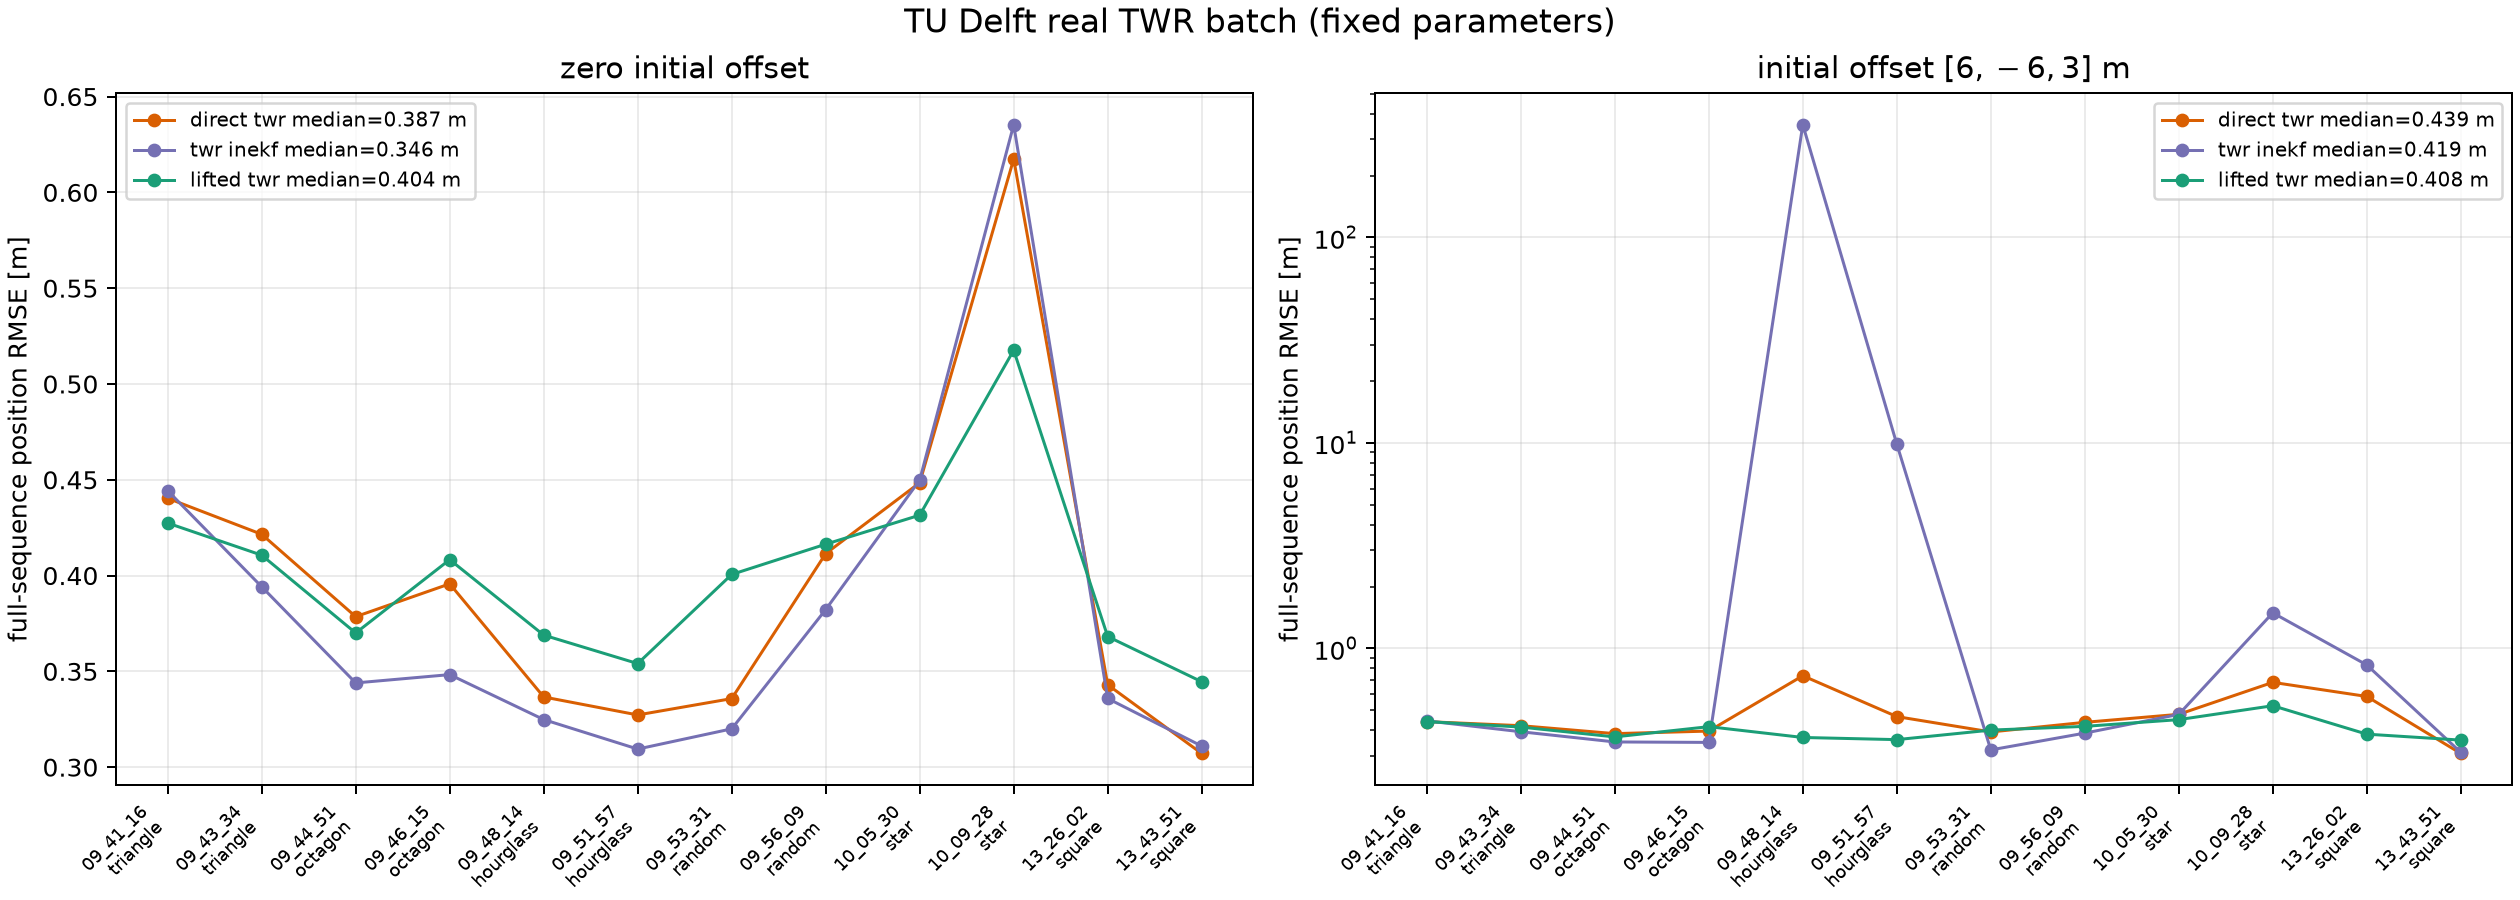
\includegraphics[width=0.98\textwidth]
{../imu-uwb-inekf-state-augment/results/task06_full/real_batch_comparison.png}
\caption{12 条真实日志的三方法批测。右图采用对数纵轴，使普通
TWR--InEKF 的两个大初差失败与其余约 0.3--0.7 m 的成功运行同时可见。}
\label{fig:real-batch}
\end{figure}

\subsection{为什么增广法末 5 s 经常更差}

12 条日志逐条比较后，原增广法有 11/12 条末 5 s 位置 RMSE 高于普通
距离 EKF，中位惩罚为 $+0.141$ m；速度末 5 s 的中位惩罚为
$+0.124$ m/s。为区分平方量测与独立辅助状态的影响，增加两个只作诊断
的消融：
\begin{enumerate}
 \item 六维平方距离 EKF：仍只估计 $[p^\top,v^\top]^\top$，使用与
       增广法相同的去偏半平方距离及距离相关方差；
 \item 投影增广法：每次接受量测后执行
 \begin{equation}
  (q,s,h)\leftarrow
  \left(\frac12p^\top p,\ p^\top v,\ v^\top v\right),\qquad
  P\leftarrow J_\Pi P J_\Pi^\top .
  \label{eq:projection-diagnostic}
 \end{equation}
\end{enumerate}
投影会使增广协方差退化回六维物理流形，因而牺牲独立 $q,s,h$ 带来的
大初差线性观测机制；它不是默认改进，只是因果消融。

\begin{center}
{\small
\textbf{末段消融（12 条真实日志、零初差）}\\[0.4em]
\begin{tabular}{lrrrr}
\toprule
方法 & 全程位置中位 & 末 5 s 位置中位 & 末 5 s 速度中位 &
末段差于直接 EKF\\
 & (m) & (m) & (m/s) & /12\\
\midrule
普通距离 EKF & 0.387 & 0.192 & 0.466 & 0\\
六维平方距离 EKF & 0.386 & 0.207 & 0.466 & 10\\
独立 $q,s,h$ 增广 & 0.404 & 0.335 & 0.565 & 11\\
增广后逐次投影 & 0.386 & 0.207 & 0.466 & 10\\
\bottomrule
\end{tabular}
}
\end{center}

投影版与六维平方距离 EKF 的 12 条末段 RMSE 最大差只有
$3.3\times10^{-16}$ m，全程 RMSE 最大差 $5.7\times10^{-4}$ m。
这说明平方变换本身仅带来约 $0.012$ m 的中位末段代价，主要额外误差
来自独立辅助状态。进一步地，末 5 s 的
$q-\tfrac12p^\top p$ RMS 与“增广减普通”的位置 RMSE 惩罚之间
Spearman $\rho=0.755$，双侧 $p=0.0045$（$n=12$）。这是小样本
相关证据，不是严格因果定理，但与投影消融相互印证。

过程噪声扫描也排除了“只把 $Q$ 调大即可解决”的解释。有效加速度标准差
从 $5,10,20,40$ m/s$^2$ 增大时，末 5 s 位置中位数依次为
$0.363,0.335,0.285,0.273$ m；但速度中位数为
$0.583,0.565,0.615,0.798$ m/s，全程位置中位数在 40 m/s$^2$ 时又升至
$0.415$ m。增大 $Q$ 只能在位置尾段与速度噪声间移动折衷，不能恢复到
物理流形版本。

\begin{figure}[H]
\centering
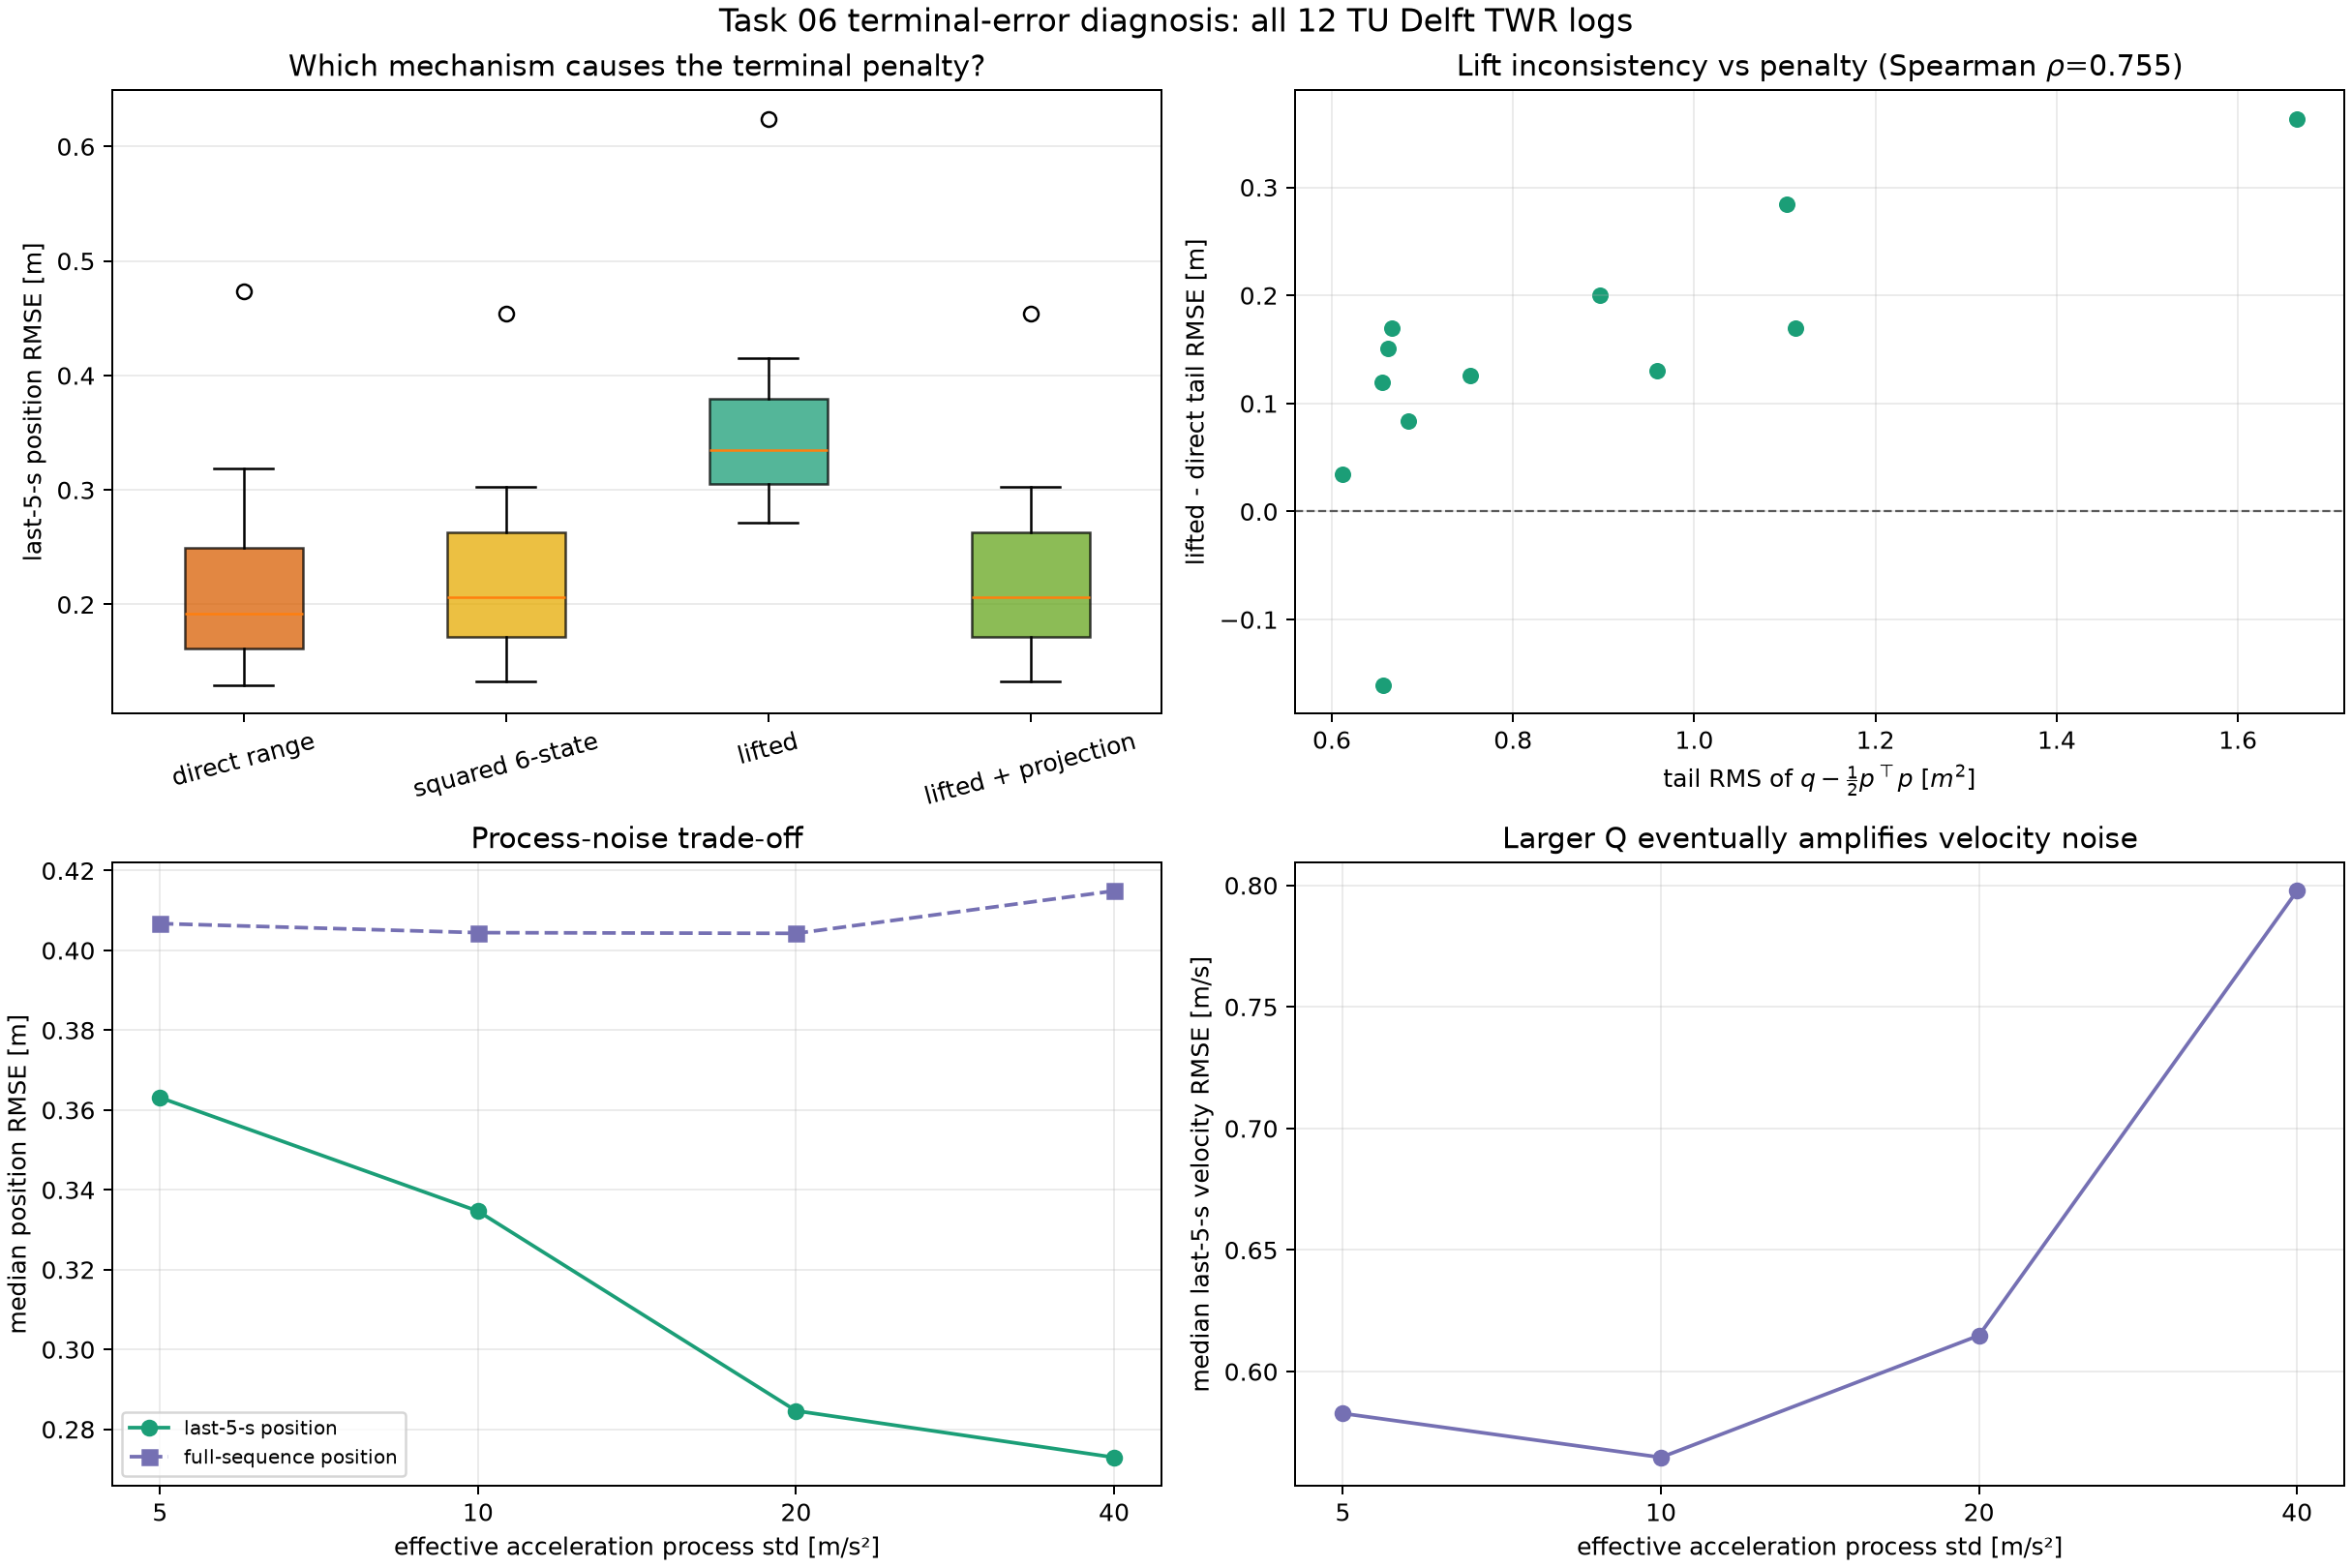
\includegraphics[width=0.98\textwidth]
{../imu-uwb-inekf-state-augment/results/task06_tail_diagnostic/tail_ablation.png}
\caption{全部 12 条日志的末段因果消融。平方量测的小幅代价、独立辅助
状态的主要惩罚、约束误差相关性及过程噪声折衷均在同图展示。}
\label{fig:tail-diagnosis}
\end{figure}

\subsection{代表性真实日志}

在 \texttt{2021-02-12\_09\_56\_09\_twr\_random.csv} 的 65.2 s、
15724 次 TWR 更新中，从 $[6,-6,3]^\top$ m 偏移开始：
\begin{table}[H]
\centering
\small
\caption{代表性随机轨迹结果。}
\begin{tabular}{lrrrr}
\toprule
方法 & 全程位置 RMSE & 末 5 s RMSE & 最大位置误差 & 速度 RMSE\\
 & (m) & (m) & (m) & (m/s)\\
\midrule
普通 TWR EKF & 0.437 & 0.167 & 3.968 & 0.803\\
增广 TWR KF  & 0.418 & 0.367 & 1.897 & 0.603\\
普通 TWR--InEKF 参考 & 0.387 & 0.188 & 3.179 & 0.425\\
\bottomrule
\end{tabular}
\end{table}
三种方法均保持有限、轨迹连续。增广法降低了全程 RMSE、最大误差和
速度 RMSE，但 $z$ 方向稳态较噪，末 5 s 指标较差。辅助状态并未强制
投影回二次流形；其 $q,s,h$ 约束 RMS 分别为
$0.442,\ 2.017,\ 1.254$（相应物理量单位），这也是当前分阶段线性
滤波器仍需改进的证据。

\begin{figure}[H]
\centering
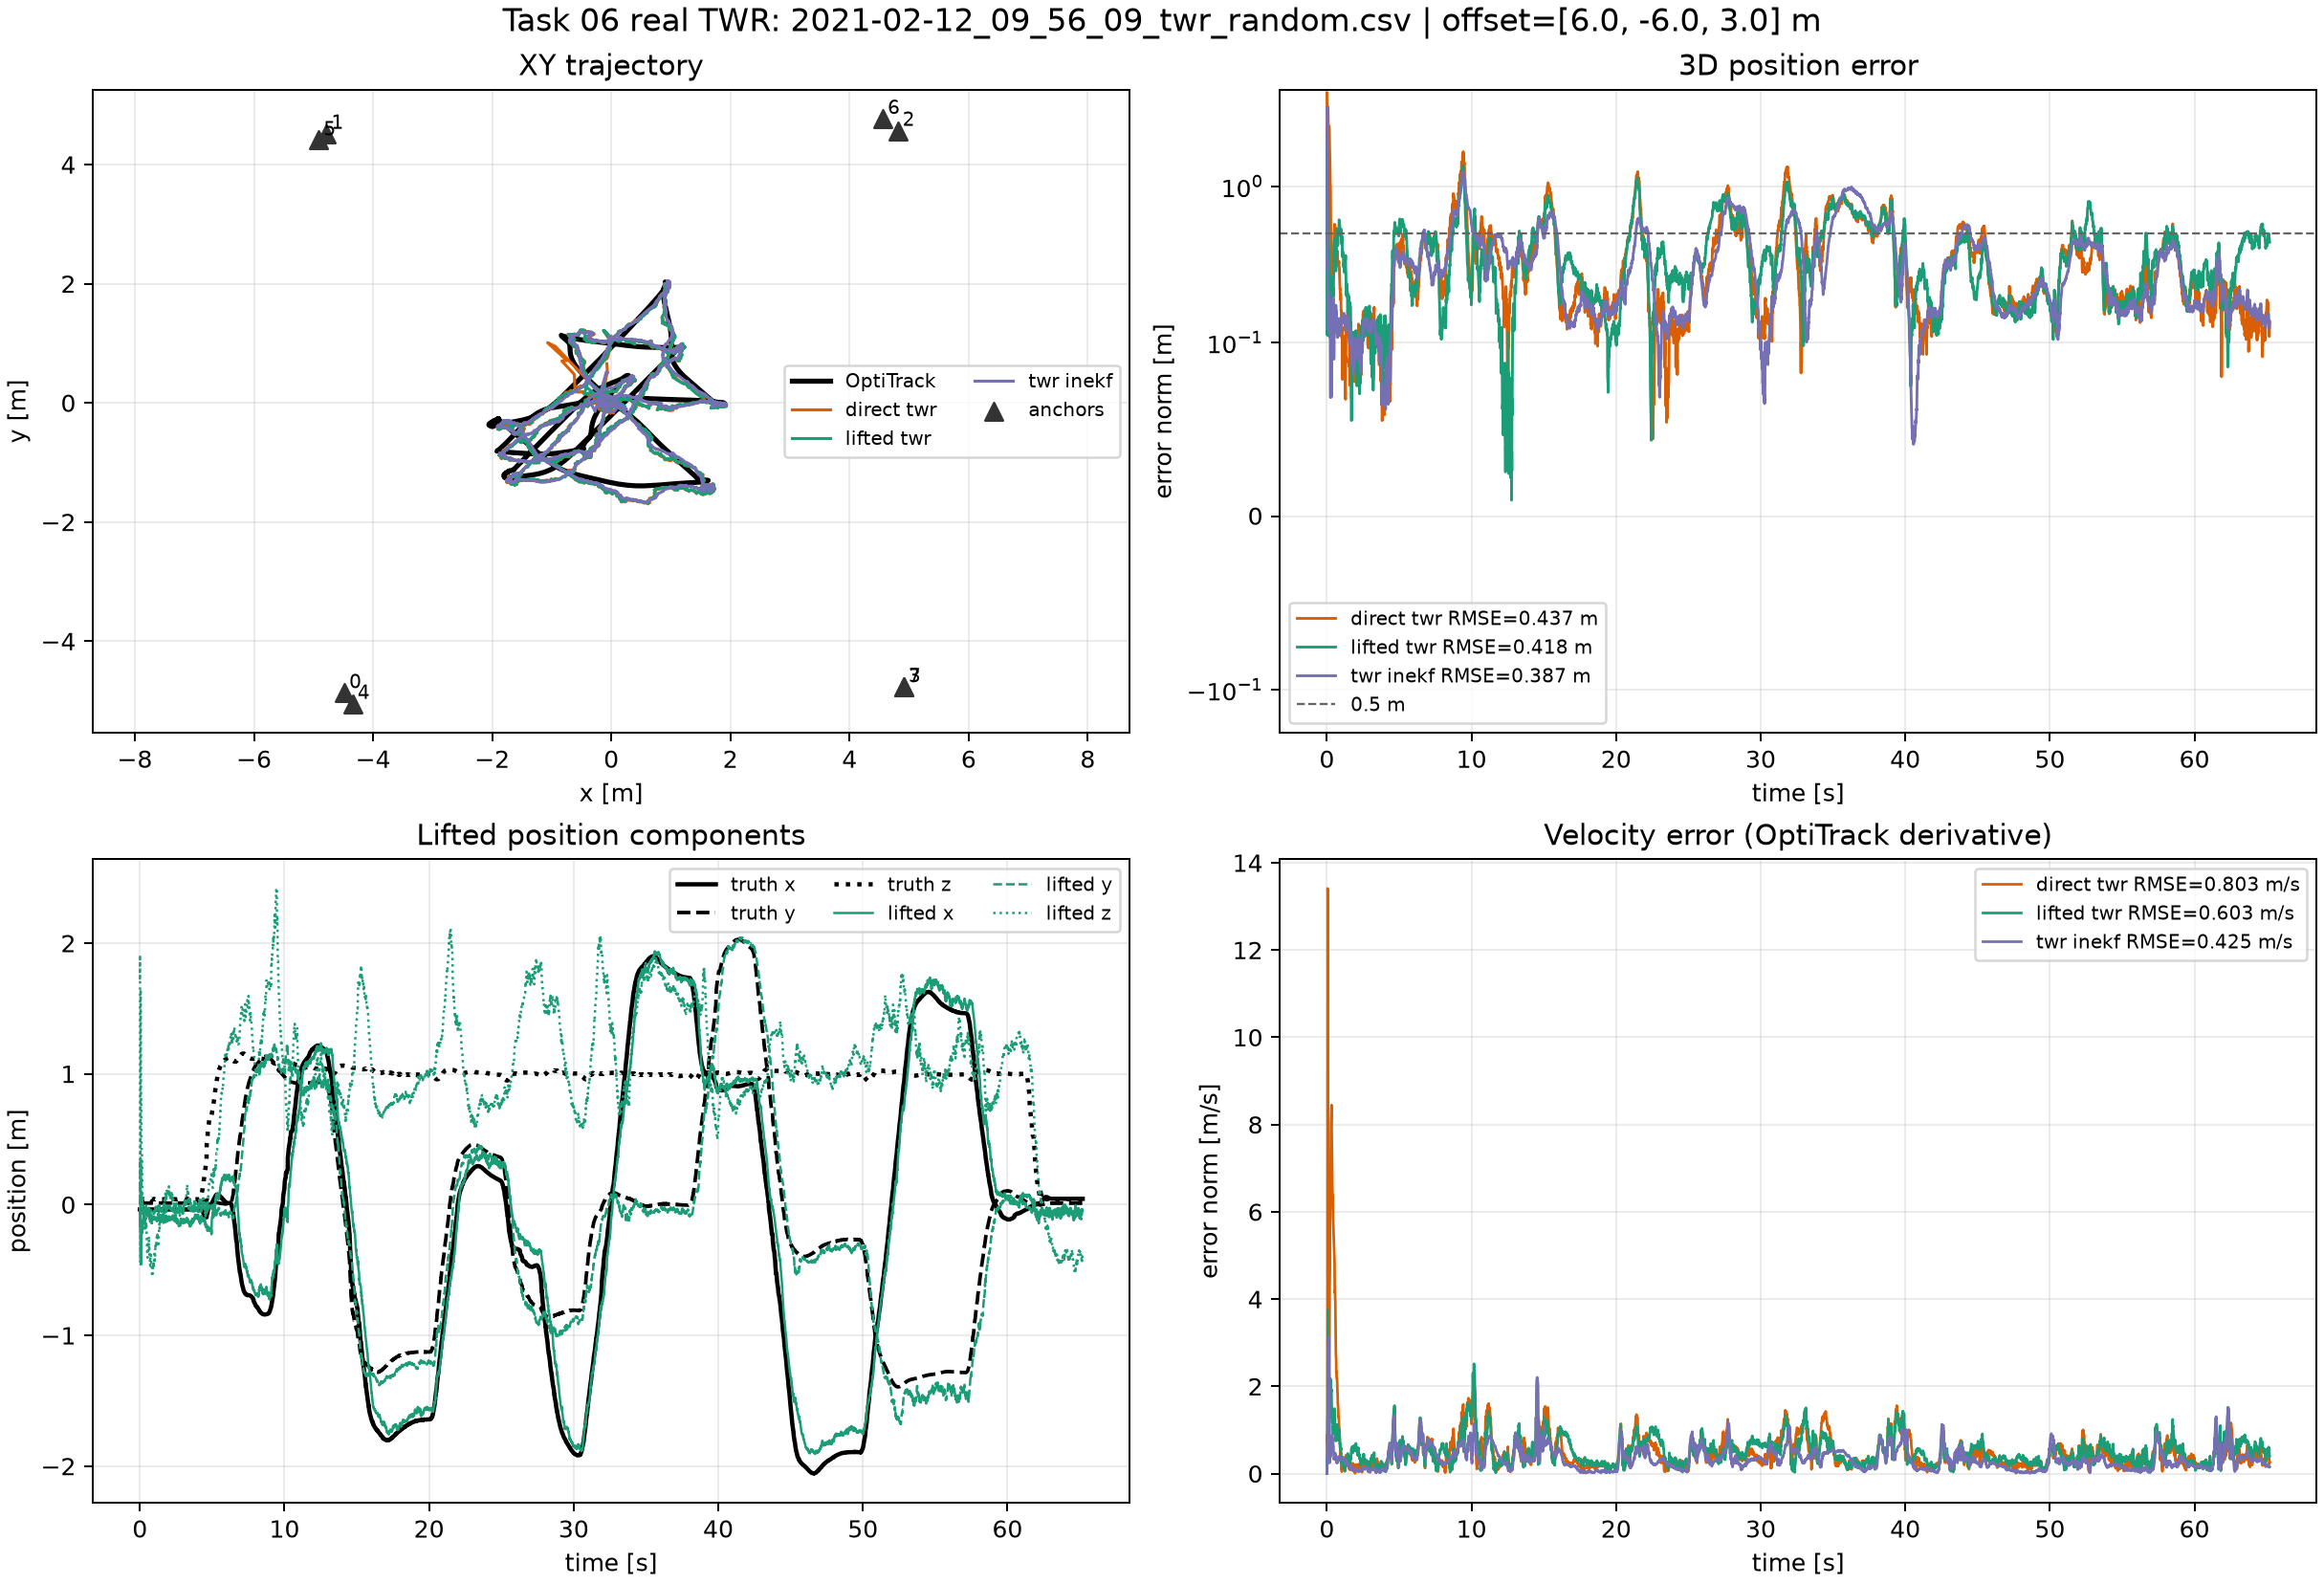
\includegraphics[width=0.98\textwidth]
{../imu-uwb-inekf-state-augment/results/task06_full/real_representative_large/comparison.png}
\caption{代表性真实轨迹。初始瞬态、分轴误差、速度误差和增广约束残差
均保留在图中。}
\label{fig:real-representative}
\end{figure}

\subsection{持续激励下的大初值合成试验}

为单独检验状态增广的结构收益，使用 Theodosis 类单锚点、已知世界系
加速度设置：
\begin{equation}
p(t)=
\begin{bmatrix}
20\cos t-20\\
10\sin(2t)+20\\
-4\cos(4t)
\end{bmatrix},
\end{equation}
并由解析式提供 $v(t),u(t)$，距离频率 20 Hz、噪声标准差 0.1 m。
为纳入普通 TWR--InEKF，使用单位姿态、已知零偏置，把同一带噪世界系
加速度换算成理想 IMU 比力。作者代码含应用相关的 $z\geq0$ 地面钳位，
故将轨迹、锚点和三种方法的坐标统一平移
$c=[0,0,100]^\top$ m；相对距离、加速度和初始误差完全不变，普通/增广
原有指标仅在 $3\times10^{-8}$ m 以下变化。三种方法统一使用前 80 次
更新不启用 NIS 门限，避免把“一开始拒绝全部量测”作为普通 InEKF 的
人为失败原因。

代表性初值 $p_0=[35,-25,20]^\top$ m 时，普通直接 EKF 末 5 s
RMSE 为 $204.4$ m，普通 TWR--InEKF 为 $151.6$ m，二者均未收敛；
增广法在 12.0 s 进入 0.5 m 范围，末 5 s RMSE 为 $0.292$ m。
增广法全程 RMSE 仍为 $19.1$ m，真实反映了约 12 s 的长初始瞬态。

\begin{figure}[H]
\centering
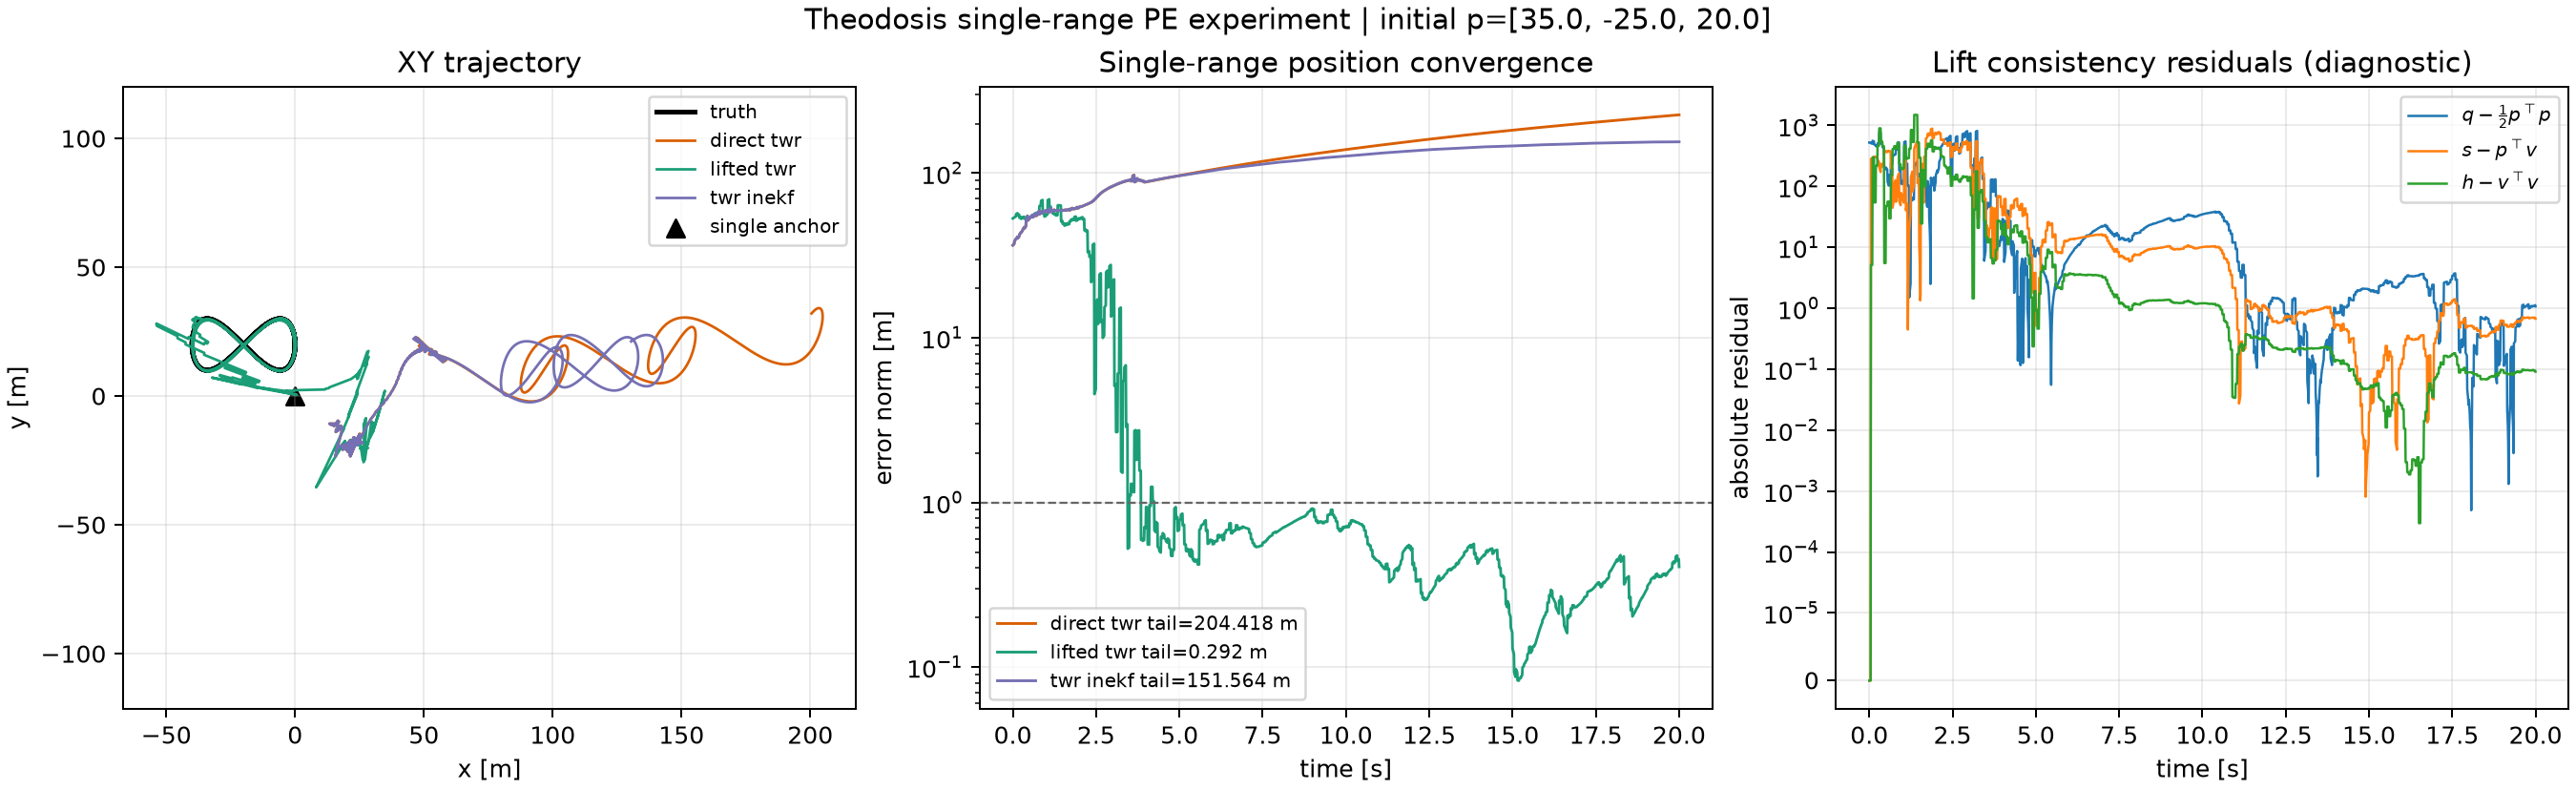
\includegraphics[width=0.98\textwidth]
{../imu-uwb-inekf-state-augment/results/task06_full/synthetic_representative/comparison.png}
\caption{单锚点持续激励代表性试验。普通直接 EKF、普通 TWR--InEKF
的发散和增广法的长收敛瞬态均未裁掉。}
\label{fig:synthetic-representative}
\end{figure}

固定随机种子 20260728，独立采样
$p_0\sim\mathcal U([-50,50]^3)$ m、
$v_0\sim\mathcal U([-10,10]^3)$ m/s，共 20 次。成功定义为末 5 s
位置 RMSE 小于 1 m：
\begin{table}[H]
\centering
\small
\caption{20 次大初值蒙特卡洛。}
\begin{tabular}{lrrrr}
\toprule
方法 & 成功数 & 成功率 & 末 5 s RMSE 中位 & 末 5 s RMSE P95\\
 & /20 & & (m) & (m)\\
\midrule
普通 TWR EKF & 0 & 0\% & 276.887 & 409.731\\
普通 TWR--InEKF & 0 & 0\% & 226.078 & 332.833\\
增广 TWR KF  & 20 & 100\% & 0.381 & 0.423\\
\bottomrule
\end{tabular}
\end{table}
普通直接 EKF、普通 TWR--InEKF、增广法的全程 RMSE 中位数分别为
$190.810,\ 164.064,\ 13.493$ m。前两者均只有预热期 80 次更新被接受，
随后 321 次因局部线性化轨迹已经偏离而被拒绝；增广法 401 次均接受。

\begin{figure}[H]
\centering
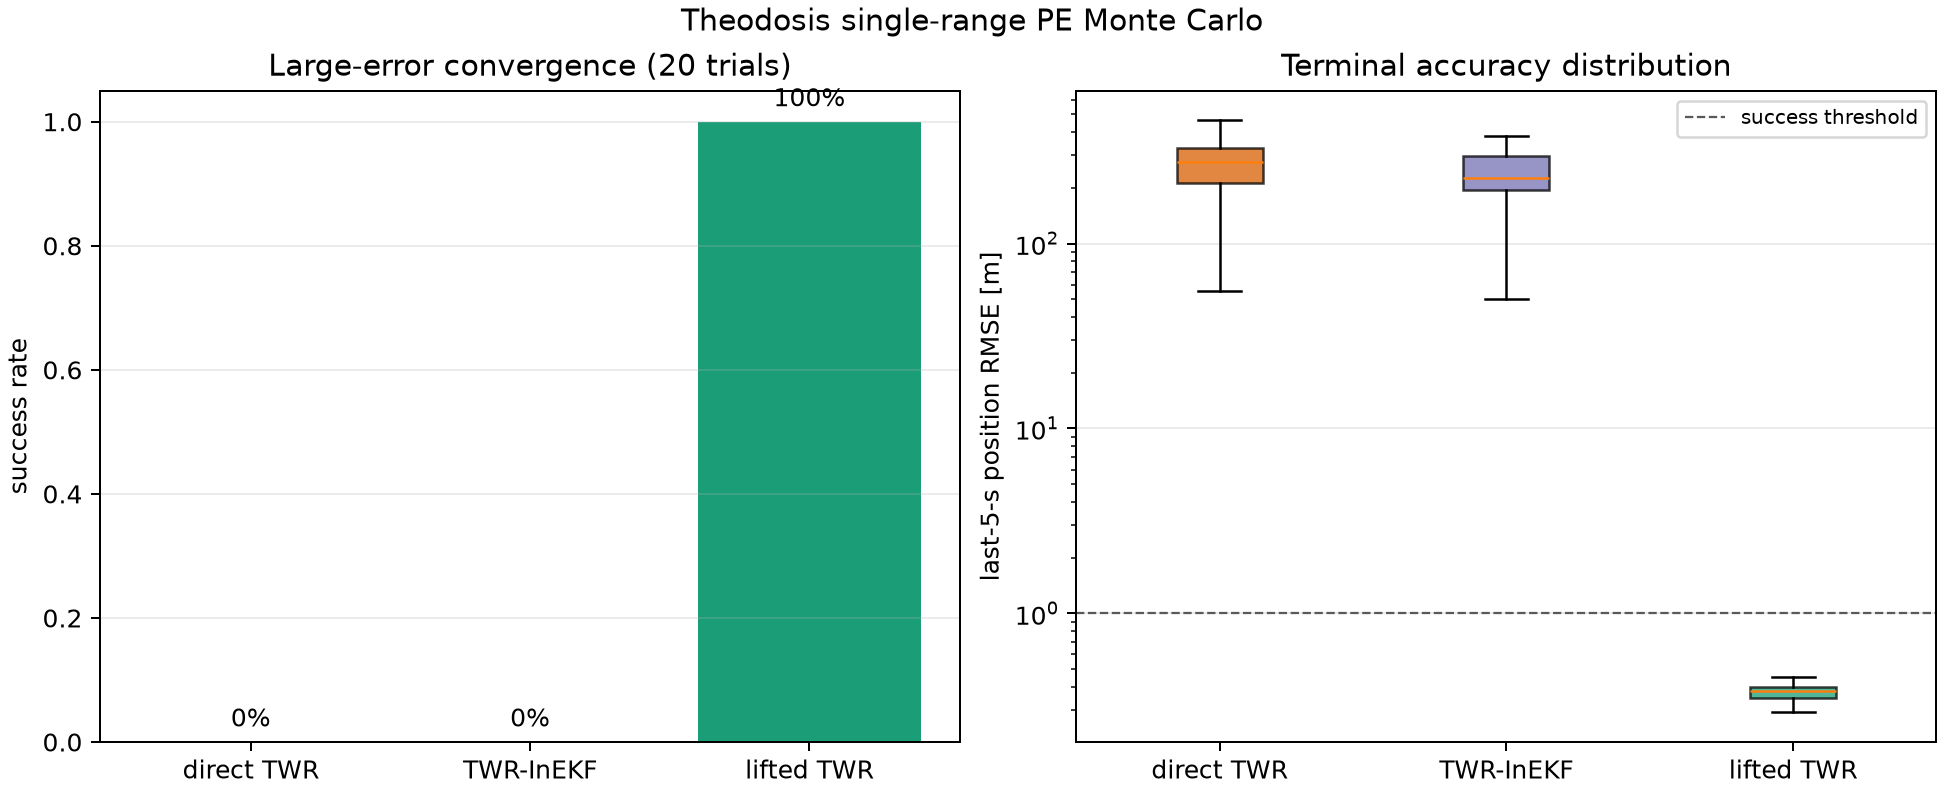
\includegraphics[width=0.98\textwidth]
{../imu-uwb-inekf-state-augment/results/task06_full/synthetic_monte_carlo/monte_carlo.png}
\caption{三方法大初值蒙特卡洛。该图只证明理想化增广平移模型在本
持续激励设置下具有更大的数值吸引域。}
\label{fig:synthetic-mc}
\end{figure}

\section{结论、限制与复现入口}

\textbf{已完成的核心目标：}TDoA 已替换为 TWR；平方距离通过
$q,s,h$ 增广进入线性状态方程；分段常值输入使用精确闭式传播；
TWR 半平方距离使用常数观测行和噪声去偏；提供普通 TWR EKF、
普通 TWR--InEKF 及增广法的可视化对照。

\textbf{证据支持的结论：}在理想化单锚点持续激励模型中，增广法显著
扩大了大初值数值收敛域；在真实多锚点数据中，大初始偏移下全程误差
和最大瞬态有所改善，但零偏移与稳态尾段没有优势。末段劣化的主要来源
已经定位为独立 $q,s,h$ 偏离二次物理流形；平方量测本身只有小幅代价，
单纯增大过程噪声又会放大速度误差。

\textbf{普通 InEKF 对照：}表 \ref{tab:real-batch} 与大初值蒙特卡洛均已
补齐普通 TWR--InEKF。它在真实零初差下中位精度最好，但大初差存在
2/12 次门限锁死；理想持续激励大初值下为 0/20。故原来只在代表性日志
给出普通 InEKF 的表格确实不完整，现已修正。

\textbf{尚未解决：}当前真实数据只有位置真值，无法验证姿态与偏置；
固定距离偏置没有建立逐锚点/NLOS 模型；UWB 不反向校正姿态和偏置；
$q,s,h$ 没有施加一致性投影；真实数据参数不是盲测得到；因此不能把
合成结果解释为高动态完整系统的全局收敛证明。诊断投影虽然改善稳态，
却删除了独立辅助自由度，不能同时冒充原增广法的大初差线性机制。

在 PowerShell 中可复现：
\begin{verbatim}
cd E:\0syncthing\Code\InEKF\imu-uwb-inekf-state-augment
.\run_task06.ps1 -Mode download
.\run_task06.ps1 -Mode test
.\run_task06.ps1 -Mode quick
.\run_task06.ps1 -Mode diagnose
.\run_task06.ps1 -Mode full
\end{verbatim}
脚本强制使用
\texttt{D:\textbackslash conda-envs\textbackslash imu-uwb-inekf}
环境，结果输出到 \texttt{results}。

\begin{thebibliography}{9}
\bibitem{oursland2024}
Oursland, J. and Mehrabian, A.,
``An Invariant Extended Kalman Filter for IMU--UWB Sensor Fusion,''
IEEE RO-MAN, 2024,
\href{https://doi.org/10.1109/RO-MAN60168.2024.10731434}
{doi:10.1109/RO-MAN60168.2024.10731434}.

\bibitem{theodosis2020}
Theodosis, P. A., et al.,
``State Estimation for a Class of Linear Systems with Quadratic Output,''
\href{https://arxiv.org/abs/2006.02688}{arXiv:2006.02688}, 2020.

\bibitem{berkane}
Berkane, S., et al.,
``Tutorial on Aided Inertial Navigation Systems:
A Modern Treatment Using Lie-Group Theoretical Methods,''
本项目参考文件 \texttt{eq\_ob.pdf}.

\bibitem{tudelft}
TU Delft,
``UWB dataset (Version 1),''
\href{https://doi.org/10.4121/14827680.v1}{doi:10.4121/14827680.v1}.
\end{thebibliography}

\end{document}
